\section{Постановка задачи}

Требуется создать систему, которая автоматически собирает описания
структуры из нескольких независимых источников, сохраняет их в едином
каталоге и предоставляет возможности для просмотра, сравнения и
объединения данных. Система должна работать как связующее звено между
источниками и не заменять их. Она не управляет бизнес-данными
источников и не требует их остановки или перестройки. Основная ценность
системы состоит в том, что она даёт единую, согласованную и актуальную
картину описаний данных, а также позволяет получать объединённые
результаты из разных источников.

Система должна подключаться к трём независимым источникам данных.
Источники могут быть разнородными по своей природе и развиваться
независимо друг от друга. Объём сведений в источниках значителен:
количество записей в каждом из них должно быть не менее 200\,000.
Система должна автоматически собирать описания структуры данных,
сохранять их в едином хранилище и вести историю изменений. Это
необходимо для того, чтобы можно было не только увидеть текущее
состояние описаний, но и сравнить его с предыдущими состояниями, а
также сопоставить описания разных источников между собой.

В состав функций системы входит:
\begin{itemize}
  \item автоматический сбор описаний структуры из всех подключённых
        источников;
  \item ведение единого каталога описаний и истории их изменений;
  \item просмотр и поиск описаний по источникам, сущностям и признакам;
  \item сравнение описаний двух источников или двух версий одного
        источника;
    \item соединение данных из разных источников по произвольным
        атрибутам;
  \item предоставление доступа к результатам через программный
        интерфейс.
\end{itemize}

Просмотр и поиск должны позволять быстро находить нужные сущности и их
признаки, не обращаясь напрямую к каждому источнику. Сравнение должно
показывать различия в составе сущностей, их признаков и связей, а также
изменения, произошедшие между версиями. Объединение данных должно
выполняться по произвольным общим признакам, даже если источники
устроены по-разному. Результат объединения должен формироваться
системой без необходимости переноса всех данных в одно хранилище и без
изменения самих источников.

Система должна хранить описания структуры в упорядоченном виде,
обеспечивающем целостность и однозначность связей между источниками,
сущностями и признаками.

\begin{figure}[htbp]
  \centering
  \resizebox{\linewidth}{!}{%
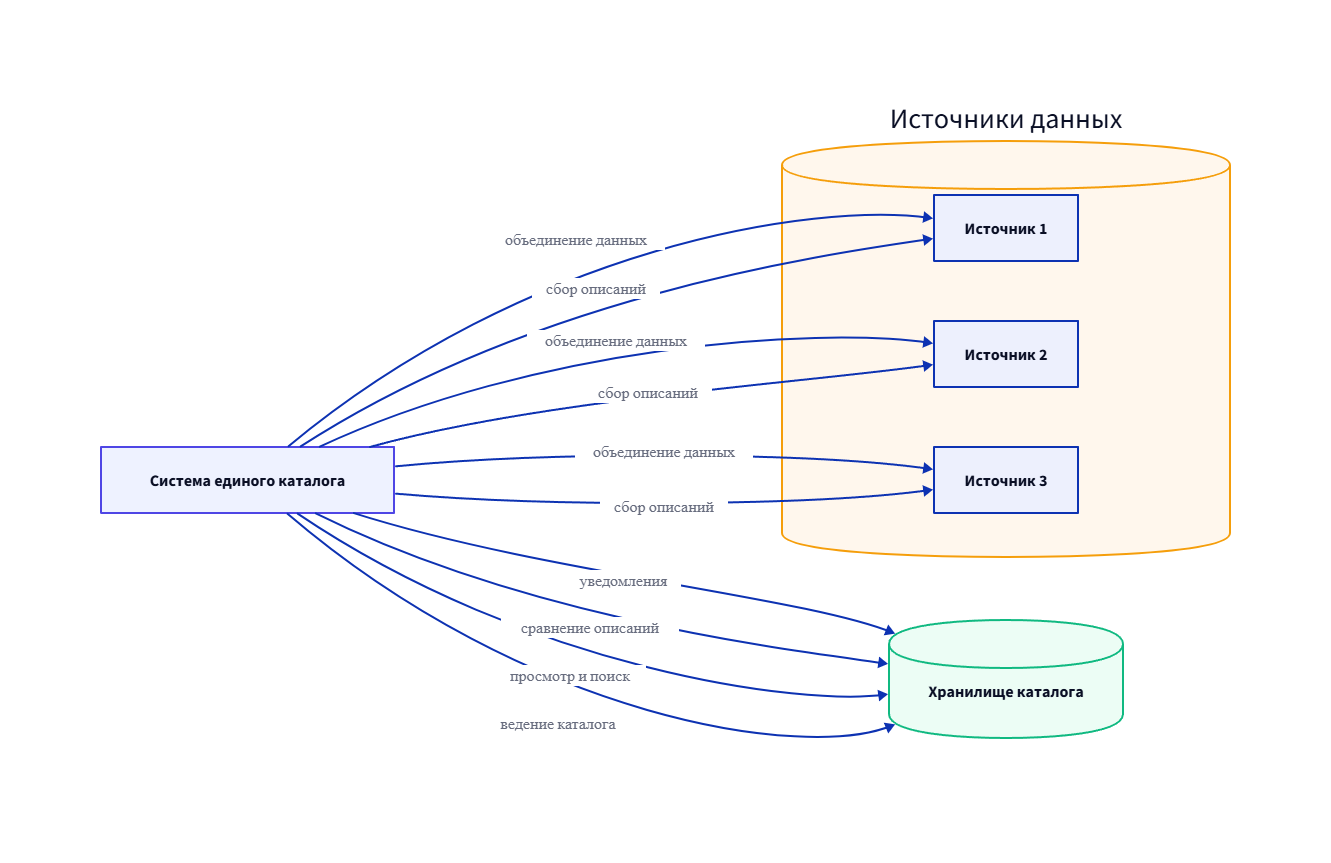
\includegraphics[width=\linewidth]{diagrams/functional.png}
  }
  \caption{Функциональная схема системы}
  \label{fig:functional}
\end{figure}